\chapter{Ход исследования}	% Заголовок

Для исследования стохастических связей между оценками параметров модели процесса при фиксированном наборе параметров алгоритма интервального оценивания, рассматривается следующая модель элементарных событий.

Для каждого модельного значения каждого параметра процесса интервальные оценки являются случайными величинами. Далее, для упрощения изложения, рассматривается одномерный случай --- параметр $\sigma$. Каждому модельному значению $s$ параметра $\sigma$ соответствуют случайные величины $\sigma_1, \sigma_2$ --- оценки границ отрезка, доставленные алгоритмом интервального оценивания. Вводится случайная величина $\omega_{(\sigma = s)}$:
  \begin{itemize}
    \item $\omega_{(\sigma = s)}(s \notin [\sigma_1, \sigma_2]) = 0$;
    \item $\omega_{(\sigma = s)}(s \in [\sigma_1, \sigma_2]) = 1$;
  \end{itemize}

Распределение вероятности $\omega_{(\sigma = s)}$ неизвестно, так как неизвестны распределения $\sigma_1, \sigma_2$. Для его аппроксимации используется эмпирический подход, причём все построения проводятся отдельно для реализаций траекторий процесса длиной в 100, 250 и 1000 элементов.

Из имеющегося множества результатов экспериментов (объёмом порядка $10^6$) извлекается информация  о попадании модельных значений параметра в оценённый отрезок: для каждого из $N$ экспериментов, в которых $\sigma = s$, величина
\[
H_{\sigma = s}^{(i)} = 1,\, i=\overline{1, N},
\]
если в $i$-ом эксперименте есть попадание, иначе она равна нулю. На основе этих выборок строится оценка параметра распределения $\omega_{(\sigma = s)}$
\[
\widehat{p}_{\sigma = s} = \P\{\, \omega_{\sigma = s} = 1\,\}
\]
согласно
\[
\widehat{p}_{\sigma = s} = \frac{1}{N} \sum_{i=1}^N H_{\sigma = s}^{(i)}.
\]

Для оценки стохастической связи между каждой парой различных $\widehat{p}$ аппроксимировались копулы их двумерных распределений. Например, пусть требуется построить копулу, соответствующую паре $\widehat{p}_{\sigma = s}, \widehat{p}_{\lambda = l}$. Тогда выбирается набор экспериментов, в которых $\sigma = s$ и одновременно $\lambda = l$, мощность множества таких результатов обозначается $M$. Выбирается размер окна $W$, равный 30 в этой работе. Далее выборка
\[
(\widehat{p}_{\sigma = s}^{(i)}, \widehat{p}_{\lambda = l}^{(i)}),\, i = \overline{1, M - W}
\]
строится так
\begin{align}
	\widehat{p}_{\sigma = s}^{(i)}  &= \sum_{k=i}^{i + W} = H_{\sigma = s}^{(k)},\, i = \overline{1, M - W} \\
	\widehat{p}_{\lambda = l}^{(i)} &= \sum_{k=i}^{i + W} = H_{\lambda = l}^{(k)},\, i = \overline{1, M - W}.
\end{align}
На основе таких двумерных выборок аппроксимируются копулы двумерного условного распределения, где условие имеет вид ${\sigma = s},  {\lambda = l}$.

Для работы с данными и выполнения вышеописанных построений используется написанный в рамках этой работы программный пакет, описанный далее.

\section*{Описание программного пакета}
\subsection*{Технический контекст}

Программный пакет представляет собой набор заголовочных файлов C++, в которых реализованы классы, необходимые для удобной работы с копулами. Созданная библиотека не использует сторонние зависимости, а значит реализации различных методов в классах, связанных с оценками, можно свободно модифицировать, не взаимодействуя с другими библиотеками.

\subsection*{Иерархия классов}

\subsubsection*{Одномерные распределения}

\begin{figure}[H]
	\centering
	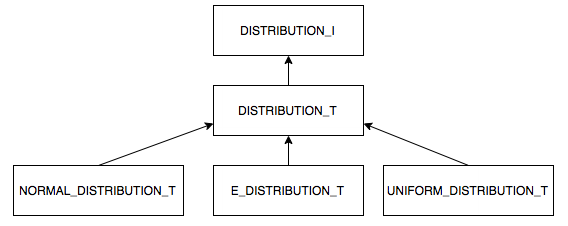
\includegraphics[width=.8\textwidth]{DIST_HIER.png}
	\caption{Иерархия классов одномерных распределений}
\end{figure}

Интерфейс \texttt{distribution\_i} предоставляет следующие возможности:
\begin{itemize}
  \item Получить значение плотности распределения в точке;
  \item Получить значение функции распределения в точке;
  \item Получить значение функции, обратной функции распределения, в точке;

  \item Получить значение мат. ожидания;
  \item Получить значение дисперсии ожидания

  \item Получить нижнюю (верхнюю) границу области определения;

  \item Вычислить предикат <<включает ли область определения свою нижнюю (верхнюю) границу>>.
\end{itemize}

Класс \texttt{e\_distribution\_t} соответствует эмпирическим распределениям, которые можно строить, импортируя выборки из внешних файлов.

Для добавления теоретических распределений, таких как \texttt{normal\_distribution\_t}, следует создать класс с \texttt{distribution\_t} в качестве предка и реализовать все необходимые методы.

\subsubsection*{Многомерные распределения}

\begin{figure}[H]
	\centering
	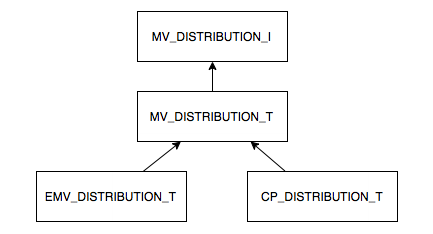
\includegraphics[width=.8\textwidth]{MV_DIST_HIER.png}
	\caption{Иерархия классов многомерных распределений}
\end{figure}

Интерфейс \texttt{mv\_distribution\_i} предоставляет следующие возможности:
\begin{itemize}
  \item Получить значение плотности распределения в точке;
  \item Получить значение функции распределения в точке;
  \item Получить значение функции распределения определённого маргинального распределения в точке;
  \item Получить значение размерности распределения.
\end{itemize}

Класс \texttt{emv\_distribution\_t} соответствует эмпирическим многомерным распределениям, которые можно строить, импортируя выборки из внешних файлов.

Для добавления теоретических распределений следует, аналогично одномерному случаю, создать класс с \texttt{mv\_distribution\_t} в качестве предка и реализовать все необходимые методы.

Класс \texttt{cp\_distribution\_t} позволяет сконструировать многомерное распределение из набора маргиналов и копулы соответствующей размерности.

\subsubsection*{Копулы}

\begin{figure}[H]
	\centering
	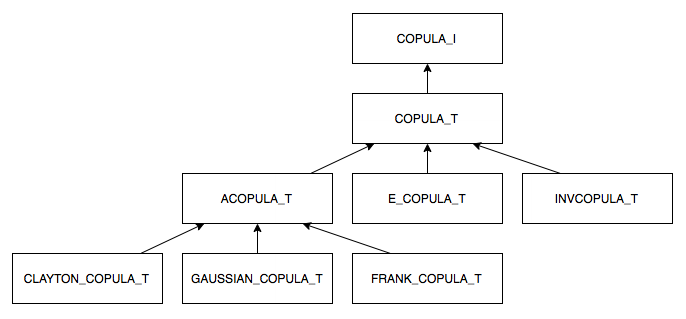
\includegraphics[width=.8\textwidth]{COPULA_HIER.png}
	\caption{Иерархия классов копул}
\end{figure}

Интерфейс \texttt{mv\_distribution\_i} предоставляет следующие возможности:
\begin{itemize}
  \item Получить значение копулы в точке;
  \item Получить значение плотности копулы в точке;
  \item Получить значение размерности копулы.
\end{itemize}

Класс \texttt{copula\_t} соответствует копулам любой размерности и объединяет своих наследников, включая в себя некоторые вспомогательные методы.

Для добавления теоретических классов копул следует создать класс с \texttt{copula\_t} в качестве предка и реализовать все необходимые методы, если это возможно. Примером может служить класс архимедовых копул, от которого так же наследуются конкретные копулы: копула Фрэнка, Гаусса и другие.

Класс \texttt{cp\_distribution\_t} позволяет сконструировать многомерное распределение из набора маргиналов и копулы соответствующей размерности.

Класс \texttt{e\_copula\_t} позволяет аппроксимировать копулы многомерных распределений, то есть экземпляров \texttt{mv\_distribution\_t}, что является одной из основных целевых возможностей библиотеки.

Чтобы получить копулу многомерного распределения наиболее простым способом --- подстановкой функций, обратных маргинальным распределениям, в многомерное --- следует использовать класс \texttt{invcopula\_t}, принимающий подобный набор параметров.

\subsubsection*{Сетка}

\begin{figure}[H]
  \centering
  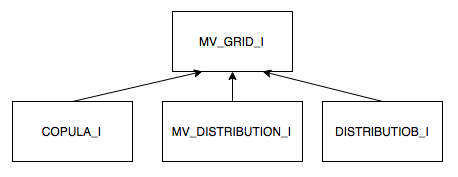
\includegraphics[width=.8\textwidth]{MV_GRID_HIER.png}
  \caption{Иерархия классов, связанных с сеткой}
\end{figure}

Все предыдущие интерфейсы делят между собой общего предка --- интерфейс \texttt{mv\_grid\_i}. Типы, соответствующие этому интерфейсу, имеют связанную с каждым экземпляром многомерную сетку. Подобные сетки используются для экспорта свойств объектов (например, плотности распределения), а также последующей визуализации.

\begin{figure}[h]
	\centering
	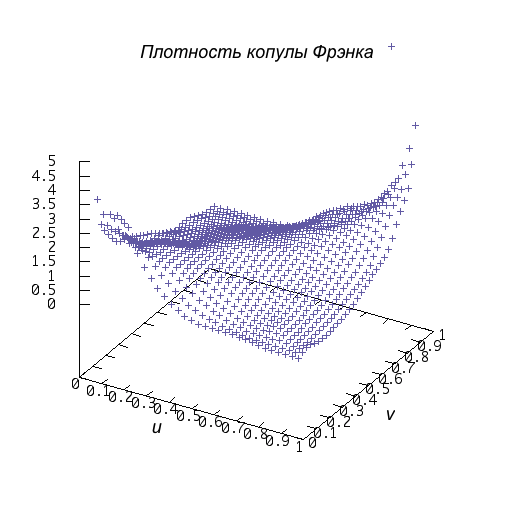
\includegraphics[width=.8\textwidth]{FRANK_GRID.png}
	\caption{Пример визуализации на сетке. Копула Фрэнка с $\tau = 0.5$.}
\end{figure}

\subsection*{Алгоритмы аппроксимации копул}

Для аппроксимации копул реализовано два алгоритма. Метод \emph{отражений}\cite{charpentier2007estimation}, работающий с двумерными распределениями, и метод \emph{преобразований}\cite{charpentier2007estimation}, позволяющий аппроксимировать копулу распределения любой размерности.

Пусть имеется выборка из двумерного распределения $(X_i, Y_i)$, содержащая $T$ элементов. Маргинальные распределения аппроксимируются в виде
\begin{align}
F_{X, T}(x) &= \frac{1}{T+1} \sum_{i=1}^T I(x - X_i) \\
F_{Y, T}(y) &= \frac{1}{T+1} \sum_{i=1}^T I(y - Y_i).
\end{align}
Знаменатель $T+1$ позволяет избежать сложностей на границах единичного квадрата, так как $F_{X, T}$ и $F_{Y, T}$ принимают значения
\[
\{\, \frac{1}{T+1}, \cdots, \frac{T}{T+1} \,\}.
\]

\subsubsection*{Метод отражений}

Для аппроксимации используются не только значения $(\widehat{U}_i, \widehat{V}_i) = (F_{X, T}(X_i), F_{Y, T}(Y_i))$, но и их отражения относительно границ и углов области определения копулы. Таким образом принимаются во внимание значения $(\pm\widehat{U}_i, \pm\widehat{V}_i), (\pm\widehat{U}_i, 2 - \widehat{V}_i), (2 - \widehat{U}_i, \pm\widehat{V}_i), (2 - \widehat{U}_i, 2 - \widehat{V}_i)$. Плотность копулы выражается в виде
\begin{equation}
  \widehat{c}_h(u, v)
  = \frac{1}{T h^2} \sum_{i=1}^T \sqts*{K\brts*{\frac{u - \widehat{U}_i}{h}}K\brts*{\frac{v - \widehat{V}_i}{h}} + \\
  % + K\brts*{\frac{u + \widehat{U}_i}{h}}K\brts*{\frac{v - \widehat{V}_i}{h}} \\
  % &+ K\brts*{\frac{u - \widehat{U}_i}{h}}K\brts*{\frac{v + \widehat{V}_i}{h}}
  % + K\brts*{\frac{u + \widehat{U}_i}{h}}K\brts*{\frac{v + \widehat{V}_i}{h}} \\
  % &+ K\brts*{\frac{u - \widehat{U}_i}{h}}K\brts*{\frac{v - 2 + \widehat{V}_i}{h}}
  % + K\brts*{\frac{u + \widehat{U}_i}{h}}K\brts*{\frac{v - 2 + \widehat{V}_i}{h}} \\
  % &+ K\brts*{\frac{u - 2 + \widehat{U}_i}{h}}K\brts*{\frac{v - \widehat{V}_i}{h}}
  % + K\brts*{\frac{u - 2 + \widehat{U}_i}{h}}K\brts*{\frac{v + \widehat{V}_i}{h}} \\
  \cdots + K\brts*{\frac{u - 2 + \widehat{U}_i}{h}}K\brts*{\frac{v - 2 + \widehat{V}_i}{h}}
  },
\end{equation}
где $K \colon \R^2 \to \R$ и $\int K = 1$.

\begin{figure}[h]
  \centering
  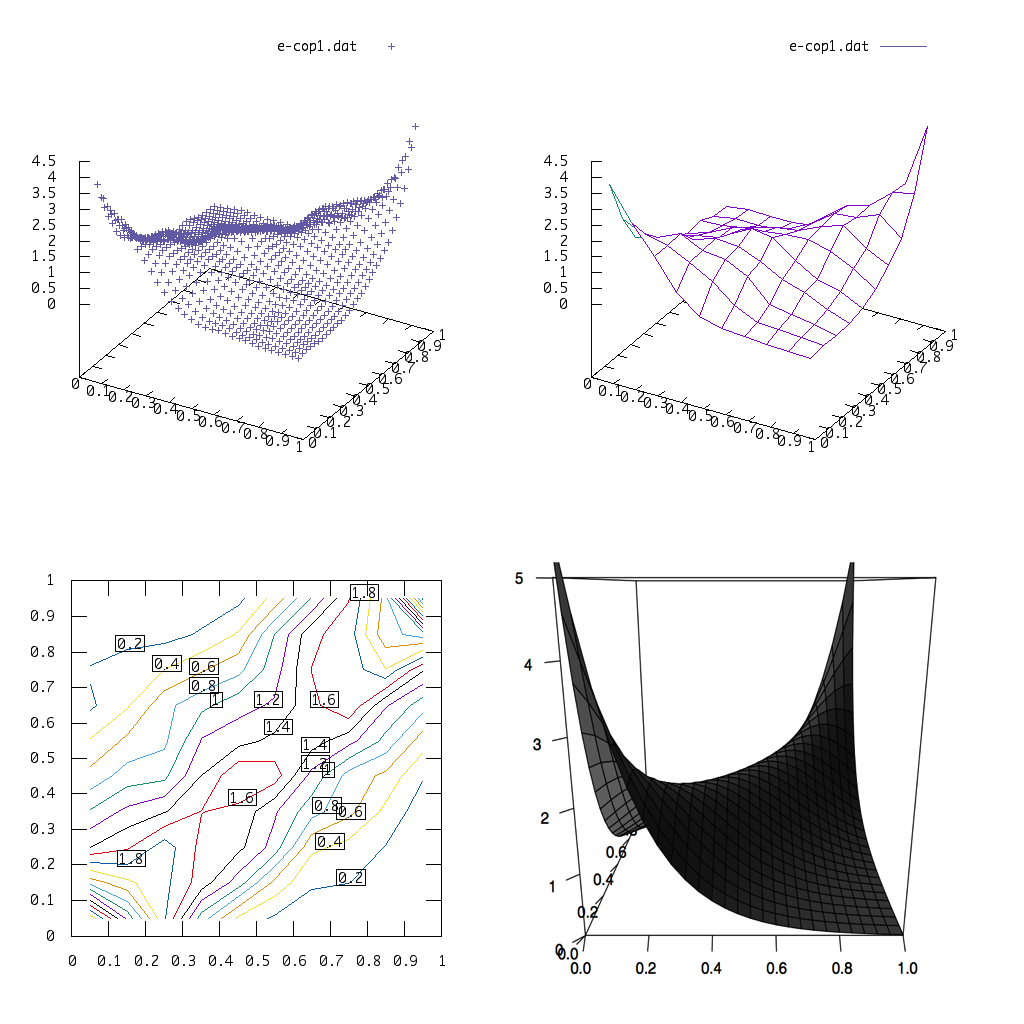
\includegraphics[width=.8\textwidth]{FrankMirror.png}
  \caption{Графики оценённой (метод отражений, 1000 наблюдений) и истинной плотностей копулы Фрэнка}
\end{figure}

\subsubsection*{Метод преобразований}

Пусть $G$ --- функция распределения непрерывного распределения на $\R$, имеющего дифференцируемую положительную плотность $g$. Известно, что величины $U = F_X(X)$ и $V = F_Y(Y)$ распределены равномерно. Тогда плотность $(\widetilde{X}, \widetilde{Y})$, где $\widetilde{X} = G^{-1}(U)$ и $\widetilde{V} = G^{-1}(V)$, равна
\begin{equation}\label{eq:transform_method}
f(x, y) = g(x)g(y)c(G(x), G(y)).
\end{equation}
Аппроксимацией этой плотности служит
\begin{equation}
\widehat{f}(x, y) = \frac{1}{T h^2} \sum_{i=1}^T K\brts*{\frac{x - \widetilde{X}}{h}, \frac{y - \widetilde{Y}}{h}},
\end{equation}
а оценка для $c$, учитывая, что из уравнения \eqref{eq:transform_method}
\begin{equation}
c(u, v) = \frac{f(G^{-1}(u), G^{-1}(v))}{g(G^{-1}(u))g(G^{-1}(v))},
\end{equation}
равняется
\begin{equation}
  \widehat{c}_h(u, v) = \frac{1}{T h^2 g(G^{-1}(u))g(G^{-1}(v))} \times \sum_{i=1}^T K\brts*{\frac{G^{-1}(u) - G^{-1}(\widetilde{U}_i)}{h}, \frac{G^{-1}(v) - G{-1}(\widetilde{V}_i)}{h}}.
\end{equation}

\begin{figure}[h]
  \centering
  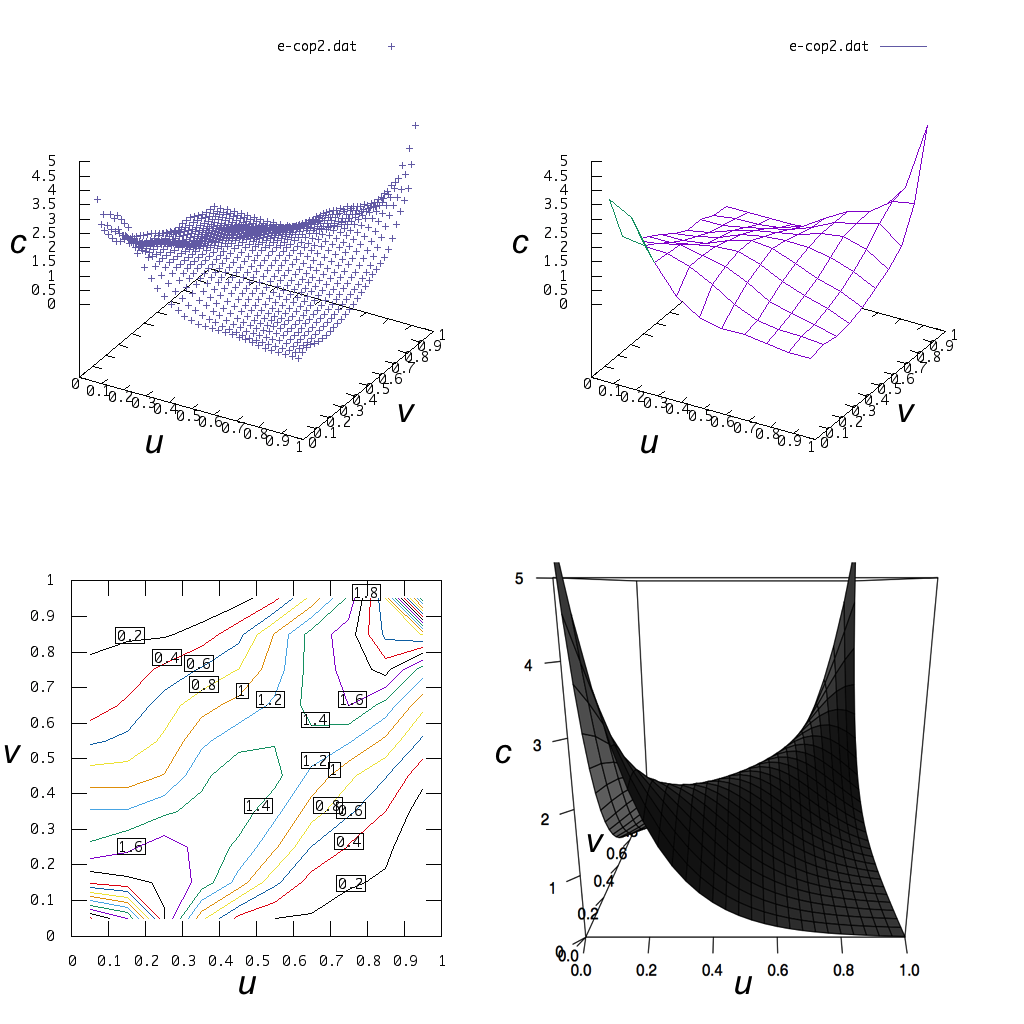
\includegraphics[width=.8\textwidth]{FrankTransform.png}
  \caption{Графики оценённой (метод преобразований, 1000 наблюдений) и истинной плотностей копулы Фрэнка}
\end{figure}

Визуализация поверхностей была осуществлена посредством экспорта соответствующих данных в формате, совместимом с входным форматом утилиты \texttt{gnuplot}.

\clearpage
